\documentclass[german, % Standardmäßig deutsche Eigenarten, englisch -> english
parskip=full, % Absätze durch Leerzeile trennen
bibliography=totoc, % Literatur im Inhaltsverzeichnis
%draft, % TODO: Entwurfsmodus -> entfernen für endgültige Version
]{scrartcl}
\usepackage{ifluatex} % zum Testen, ob LuaTeX verwendet wird
\ifluatex
\usepackage{fontspec} % Laden von Schriften
\setmainfont[Mapping=tex-text]{Linux Libertine O}  % Mapping ermöglicht die Verwendung z.B. von --
\setsansfont[Mapping=tex-text]{Linux Biolinum O}
\usepackage{polyglossia}  % Sprachpaket
\setdefaultlanguage[spelling=new,babelshorthands=true]{german}  % Neue Rechtschreibung und Abkürzungen
\else % kein LuaTeX
\usepackage[utf8]{inputenc} % Kodierung der Datei
\usepackage[T1]{fontenc} % Vollen Umfang der Schriftzeichen
\usepackage{lmodern}
\usepackage[ngerman]{babel} % Sprache auf Deutsch (neue Rechtschreibung)
%\usepackage{libertine} % Schriftart Linux Libertine/Biolinum verwenden
\fi

% Mathematik und Größen
\usepackage{amsmath}
\ifluatex
\usepackage{unicode-math}
\fi
\usepackage[locale=DE, % deutsche Eigenarten, englisch -> US
separate-uncertainty, % Unsicherheiten seperat
]{siunitx}
\usepackage{physics} % Erstellung von Gleichungen vereinfachen

% Bilder einbinden
\usepackage{graphicx}
\usepackage{float}
\usepackage{caption}
%\graphicspath{{bilder/}} % TODO: Pfad unter dem die Bilder gesucht werden

% Gestaltung
\usepackage{microtype}  % Mikrotypographie
\usepackage{booktabs}  %schönere Tabellen
\usepackage{multirow}
\usepackage[toc]{multitoc}  %mehrspaltiges Inhaltsverzeichnis
\usepackage{csquotes} % Anführungszeichen mit \enquote
\usepackage{subcaption}  % Unterabbildungen a,b,c,…
\usepackage{enumitem}  % Listen anpassen
\setlist{itemsep=-10pt}
\usepackage{scrpage2}  % Manipulation des Seitenstils
% Kopf-/Fußzeilen
\pagestyle{scrheadings}
\clearscrheadings
\automark{section}
\ofoot{\pagemark}
\ihead{\headmark}
\setheadsepline{.5pt}

\usepackage[colorlinks=true]{hyperref}  % Links und weitere PDF-Features

\makeatletter 
\renewcommand\subsection{\@startsection 
   {subsection}{2}{0mm}%      % name, ebene, einzug 
   {0.5\baselineskip}%            % vor-abstand 
   {0.3\baselineskip}%            % nach-abstand 
   {\bfseries\sffamily\large}%           % layout 
   } 
\makeatother 

% TODO: Titel und Autor, … festlegen
\newcommand*{\titel}{Mößbauerspektroskopie}
\newcommand*{\autor}{Maximilian Obst, Thomas Adlmaier}
\newcommand*{\abk}{MBS}
\newcommand*{\betreuer}{Philipp Materne}
\newcommand*{\messung}{18.11.2016}
\newcommand*{\ort}{Technische Universität Dresden, Institut für Festkörperphysik}

\hypersetup{pdfauthor={\autor}, pdftitle={\titel}} % PDF-Metadaten

\titlehead{F-Praktikum \abk \hfill TU Dresden}
\subject{Versuchsprotokoll}
\title{\titel}
\author{\autor}
\date{\begin{tabular}{ll}
Protokoll: & \today\\
Messung: & \messung\\
Ort: & \ort\\
Betreuer: & \betreuer\end{tabular}}

%----------------
\begin{document}
\begin{titlepage}
\maketitle

\begin{figure}[hb] 
  \centering
     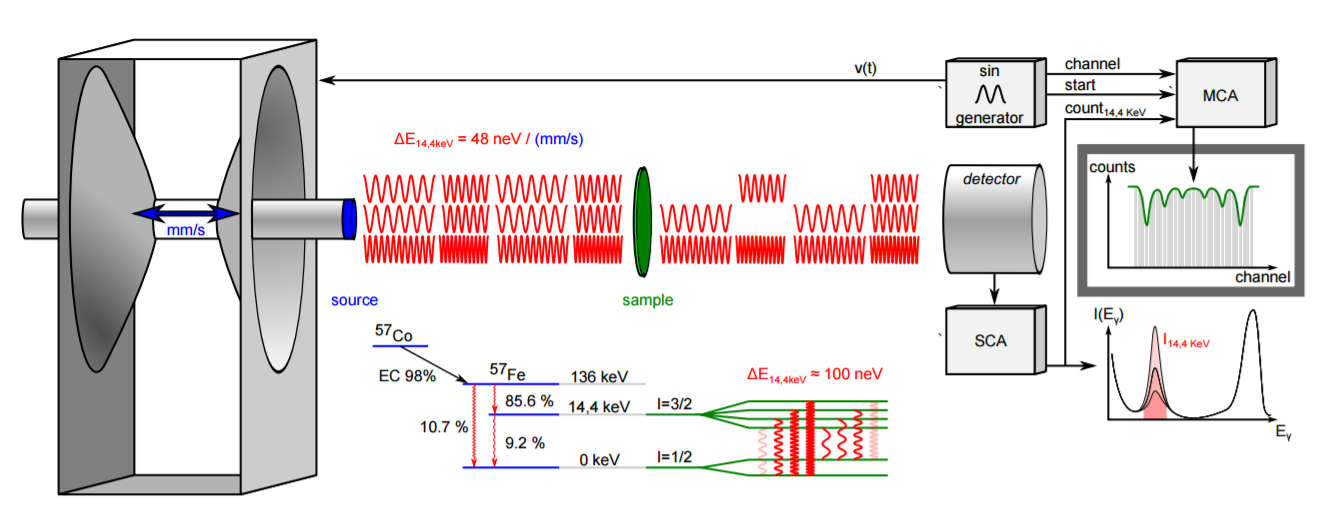
\includegraphics[width=0.8\textwidth]{moessbauer}
  \caption{Aufbau und Funktionsprinzip der Mößbauerspektroskopie an \textsuperscript{57}Fe \cite{skript}}
  \label{fig:moessbauer}
\end{figure}
\end{titlepage}

\tableofcontents
\pagebreak

%------------------------
\section{Physikalische Grundlagen}

Die Mößbauerspektroskopie ist ein physikalisches Analyseverfahren, bei dem zerstörungsfrei ein Material auf seine Bestandteile sowie ihre elektrische Interaktion untersucht wird. Das Hauptanwendungsgebiet ist dabei die Unterscheidung zwischen zwei- und dreiwertigem Eisen. \cite{basic}
Für die Mößbauerspektroskopie werden sowohl der Doppler- als auch der Mößbauer-Effekt genutzt.

\subsection{Hyperfeinwechselwirkungen}

\begin{figure}[hb] 
  \centering
     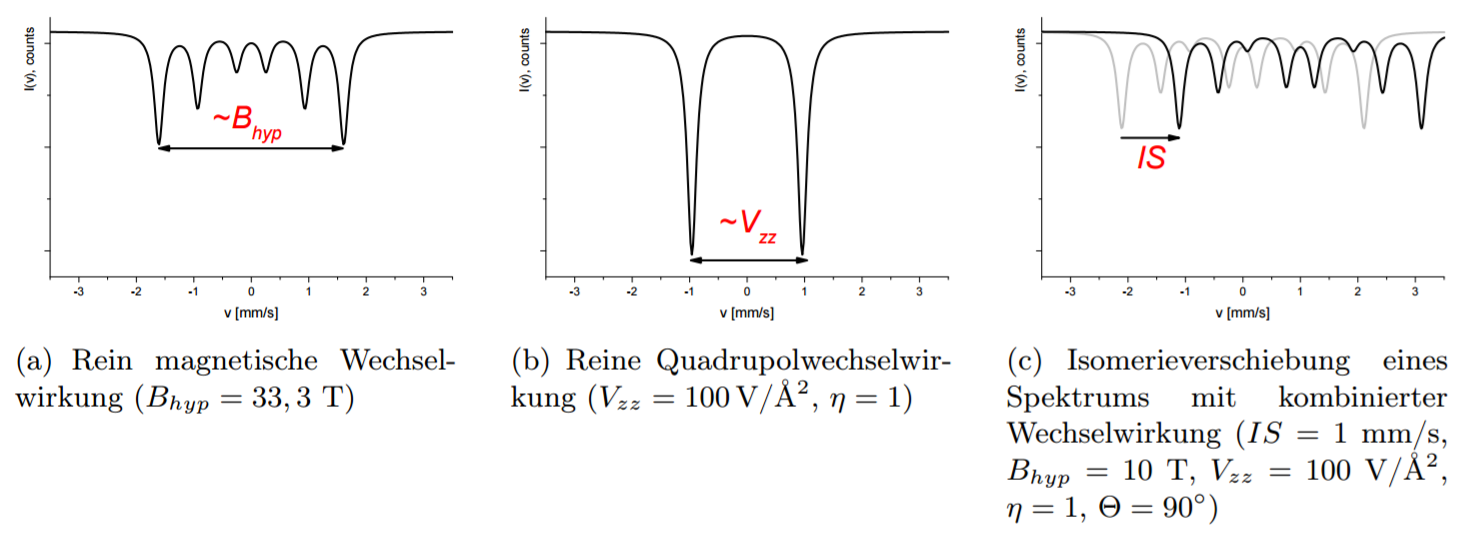
\includegraphics[width=0.8\textwidth]{GraphMoessbauer}
  \caption{Hyperfeinwechselwirkungen von \textsuperscript{57}Fe \cite{skript}}
  \label{fig:graphmoessbauer}
\end{figure}

Die Hyperfeinstruktur ist eine Aufspaltung der Energieniveaus in den Spektrallinien der Atomspektren und damit einer der Effekte, die der Entartung entgegenwirken. Sie ist etwa 2000 mal kleiner als die Feinstruktur und wird durch die Interaktion der Elektronen mit dem Kernspin, die in elektrische und magnetische unterschieden werden können, und den verschiedenen Isotopen eines Atoms bewirkt. \cite{hyperfein}

\subsubsection{Magnetischer Kernspineffekt}

Der magnetische Kernspineffekt führt zur sogenannten Zeeman-Aufspaltung: Dabei wird das Spektrum in $2I+1$ Zustände geteilt. Für \textsuperscript{57}Fe kann das Zeeman-Spektrum in Bild \ref{fig:graphmoessbauer}(a) gesehen werden.  
\begin{align}
H_z = -g_I \mu_n I_z B_z \label{for:magKSpin}
\end{align}

\subsubsection{Elektrische Kernspineffekte}

Die Effekte des elektrischen Kernpotentials lassen sich über folgende Formel verstehen:

\begin{align}
H_{elektr.} = \int \rho (\vec r) \Phi (\vec r) d^3 \label{for:eleKSpin}
\end{align}
Diese Formel kann mit einer Taylorreihe entwickelt werden:
\begin{align}
H_{elektr.} \approx Z e \Phi (0) - \frac{Z e < r^2 > \rho_e (0)}{6 \epsilon_0} + \frac{e}{6}\sum_i^3 V_{ii} Q_{ii} \label{for:eleKSpin_f}
\end{align}

Hierbei beschreibt der erste Teil die normalen Kernzustände, der zweite eine Isomerieverschiebung und der dritte das Quadropolmoment. Die Isomerieverschiebung beschreibt dabei die Energie des Kerns in der Elektronenhülle. Da sie nur von Größen aufgestellt wird (Ladungsdichte der Hülle $\rho_e$ und Kernsradius $<r^2>$, die für das ganze Atom gelten, verschiebt sie alle Übergangsenergien in gleichem Maß, wie in Bild \ref{fig:graphmoessbauer}(c) gesehen werden kann. Da eine Isomerieverschiebung auch in der Strahlungsquelle auftreten kann, muss sie stets auf die Quelle bezogen werden. Das Quadropolmoment schließlich lässt im Sonderfall, dass $V_{xx} = V_{yy}$ darauf schließen, wie groß der Kernspin ist: Bei einem Kernspin von $\frac{1}{2}$ entsteht keine Aufspaltung, bei $\frac{3}{2}$ wird das Spektrum schon in zwei Zustände geteilt - dieser Fall tritt bei \textsuperscript{57}Fe auf und das entstehende Bild kann in Bild \ref{fig:graphmoessbauer}(b) gesehen werden. Dies ist darauf zurückzuführen, dass im genannten Sonderfall das Quadropolmoment nur vom Quadrat der z-Richtung der Hauptquantenzahl $I_z$ abhängig ist.

\subsubsection{Isotopeneffekte}

\begin{itemize}
\item \textbf{Kernmassen-Effekt} Bei Absorption und Emission von Photonen durch Atome findet eine Auslenkung der Atomkerne von ihrer Ruhelage statt. Dies führt zu einer Schwingung, die die effektive Masse der Elektronen absenkt. Das wiederum führt zu einer Ausspaltung der Energieniveaus, die von der Masse des Atomkerns und somit dem Isotop abhängt. Dieser Effekt wird bei steigender Kernmasse geringer.
\item \textbf{Kernvolumen-Effekt} Elektronen der s-Schale haben eine große Wahrscheinlichkeit, sich im Atomkern zu befinden. Dies führt zu einer Abweichung des Potentials, was eine Anhebung der Energieniveaus zur Folge hat. Dieser Effekt wird größer, ja größer der Kern wird, die Abweichung bei verschiedenen Isotopen ist aber bei kleinen Kernen größer, da hier die Volumendifferenzen stärker ins Gewicht fallen.
\end{itemize}

\subsection{Mößbauereffekt}

Wie unter Isotopeneffekte beschrieben, beginnt ein Atomkern zu schwingen, sobald er ein Photon emittiert oder absorbiert. Diese Schwingung ist von der Energie des Photons und der Masse des Atomkerns abhängig. Der Mößbauereffekt jedoch beseitigt diese Effekte nahezu vollständig: Bestimmte Elemente sind in der Lage, den entstehenden Stoß über das gesamte Gitter zu verteilen. Damit ist der Anteil der Masse des Atomkerns um Größenordnungen höher. Der Stoß wird damit nahezu rückstoßfrei.

\subsection{Dopplereffekt}

Der Doppler-Effekt beschreibt die Dehnung oder Stauchung von Wellen, die durch eine Bewegung des Wellen-Aussenders hervorgerufen werden. Beschrieben wird der Effekt häufig über die entstehende Frequenzänderung. Ohne Medium, also für elektromagnetische Wellen, kann diese Änderung mit folgenden Formeln beschrieben werden:
\begin{align}
f_{Beobachter;allgemein} = f_{Quelle} \frac{\sqrt{1 - \frac{v^2}{c^2}}}{1 - \frac{v}{c} \cos (\alpha)} \\
f_{B; longitudinal} = f_{Quelle} \sqrt{\frac{c + v}{c - v}} \\
f_{B; transversal} = f_{Quelle} \sqrt{1 - \frac{v^2}{c^2}} \label{for:doppler}
\end{align}
Dabei beschreibt $\alpha$ den Winkel zwischen Bewegung und der Strecke Beobachter-Quelle.

\subsection{Radioaktiver Zerfall}

Nicht alle Atomkerne sind stabil. Einige können zerfallen. Dieser Zerfall ist je nach Atomkern unterschiedlich, es werden vier Arten unterschieden:

\textbf{Alpha-Strahlung:} Hier werden beim Zerfall des Atomkerns He\textsuperscript{2+}-Kerne freigesetzt. Diese sind sehr schwer und können daher schwere Schäden in ihrer Umgebung anrichten. Allerdings fliegen diese Teilchen nicht sehr weit und können gut abgeschirmt werden.
\begin{align}
{}^A_Z\mathrm{X} \to {}^{A-2}_{Z-2}\mathrm{Y} + {}^2_2\mathrm{He} \label{for:alpha}
\end{align}

\textbf{Beta-Strahlung:} Bei dieser Strahlungsart wandelt sich ein Neutron in ein Proton oder umgekehrt. Die entstehenden Elektronen oder Positronen fliegen weiter als Alpha-Teilchen, haben aber auch eine verringerte schädingende Wirkung.
\begin{align}
{}^A_Z\mathrm{X} \to {}^{A}_{Z+1}\mathrm{Y} + e^- + \bar \nu_e \\
{}^A_Z\mathrm{X} \to {}^{A}_{Z-1}\mathrm{Y} + e^+ + \nu_e \label{for:beta}
\end{align}

\textbf{Gamma-Strahlung:} Diese Strahlung führt nicht zu einer Veränderung des Atomkerns sondern bringt diesen nur von einem angeregten Zustand zurück in den Grundzustand. Dabei werden hochenergetische Photonen ausgesendet, die nur schwach schädigend wirken, aber eine hohe Reichweite haben und kaum abzuschirmen sind.
\begin{align}
{}^A_Z\mathrm{X*} \to {}^{A}_{Z}\mathrm{X} + \gamma \label{for:gamma}
\end{align}

\section{Durchführung}

Im Versuch wird eine ummantelte \textsuperscript{57}Co-Quelle verwendet, die Gammastrahlung emittiert. Die Energie der emittierten Photonen haben Peaks bei $136\,keV$, $122\,keV$ und $14.4\,keV$. Für die Messung sind Photonen der Energie $14.4\,keV$ interessant. Für die Detetktion wird ein Silicium-Detektor verwendet.
Ziel des Versuchs ist eine Einführung in die Verwendungsmethoden von lokalen Sonden, im speziellen der Mößbauer-Spektroskopie.

\subsection{Kalibrierung}

Um die Messung möglichst genau zu machen, soll das Programm nur Photonen aufzeichnen, die im gewollten Energiespektrum liegen. Dafür muss am Anfang das Gamma-Fenster auf den $14.4\,keV$-Peak gesetzt werden. Um diesen zu bestimmen, wird je eine 5-minütige Messung des Pulshöhenspektrums von der Quelle ohne Probe und mit einer $4x3\,\mu m$-Eisenfolie aufgenommen. Die Spektren werden übereinandergelegt und aus dem entstehenden Bild der $14.4\,keV$-Peak bestimmt. Anschließend wird das Gammafenster auf diesen Peak gesetzt.

Danach wird das Mößbauer-Spektrum der $4x3\,\mu m$-Eisenfolie etwa 75 Minuten lang aufgenommen. Dafür wird eine Spannung $U_{Antrieb}$ von etwa $195\, mV$ an den Antrieb der \textsuperscript{57}Co-Quelle angelegt. Mithilfe des aufgenommenen Spektrums wird der $\alpha$-Faktor zwischen $U_{Antrieb}$ und Geschwindigkeit $v_{Quelle}$ bestimmt. Dafür wird das Programm Moessfit verwendet, welches mit einem ersten abgeschätzen $\alpha$-Faktor einen Fit an das Mößbauer-Spektrum anlegt und einen dafür passenden Wert des Magnetfeldes zwischen den Atomen $B_{fit;Atome}$ angibt. Mit dem Wissen, dass das Magnetfeld zwischen den Atomen $B_{th.;Atome}$ $33.3\,T$ entsprechen soll, wird über die Formel \ref{for:alphafaktor} der korrekte $\alpha$-Faktor bestimmt. Anschließend werden die in Moessfit zur Verfügung stehenden Variablen angepasst, bis das verwendete Modell bestmöglich dem betrachteten Verhalten entspricht. Die Anpassungen werden physikalisch erklärt.
\begin{align}
v_{Quelle} = \alpha_{exp} U_{Antrieb} \\
\alpha_{exp} = \alpha_{Schätzung} \frac{B_{th.;Atome}}{B_{fit;Atome}} \label{for:alphafaktor}
\end{align}

\subsection{Eisenfolie}

Nun wird das Mößbauer-Spektrum einer $25\,\mu m$-Eisenfolie wieder über etwa 75 Minuten aufgenommen. Im aufgenommenen Bild werden wieder die Variablen angepasst, bis das Modell bestmöglich übereinstimmt. Anschließend wird das betrachtete Spektrum mit dem der $4x3\,\mu m$-Eisenfolie verglichen und die Abweichungen physikalisch erklärt.

\subsection{Ferrocen}

Der Versuch wird ein weiteres Mal für Ferrocen durchgeführt. Dabei wird eine verringerte Antriebsspannung verwendet, die eine Geschwindigkeit der Quelle von $2.5\,mm/s$ bewirkt. Wieder werden im aufgenommenen Bild die Variablen angepasst und die Anpassungen physikalisch erklärt.

\subsection{Auswirkungen eines Magnetfeldes}

Im letzten Versuchsteil werden an die $25\,\mu m$-Eisenfolie zwei unterschiedliche Magnetfelder angelegt, wieder über etwa 75 Minuten das Mößbauer-Spektrum aufgenommen und in den erhaltenen Bildern die Variablen angepasst, bis das Modell die Werte am Besten wiedergibt. Die Bilder und Variablen werden miteinander und mit den Bildern und Variablen der anderen Eisenfolien-Messungen verglichen und die Ergebnisse physikalisch interpretiert.  

\section{Analyse}


\section{Fazit}



%------------------------

\begin{thebibliography}{9}

\bibitem{skript}
  https://tu-dresden.de/mn/physik/ifp/ressourcen/dateien/lehre/praktika/mbs?lang=de
	16.11.2016
	16:00 Uhr
	
\bibitem{basic}
  https://de.wikipedia.org/wiki/M\%C3\%B6\%C3\%9Fbauerspektroskopie
	16.11.2016
	16:15 Uhr
	
\bibitem{hyperfein}
  https://de.wikipedia.org/wiki/Hyperfeinstruktur
	16.11.2016
	16:15 Uhr
	
\bibitem{doppler}
  https://de.wikipedia.org/wiki/Doppler-Effekt\#Doppler-Effekt\_ohne\_Medium
	16.11.2016
	17:50 Uhr

\end{thebibliography}

\end{document}
